
\chapter{Présentation}
\label{chapter:poodlePres}

L'attaque Poodle\up{\cite{article:ssl-poodle2}} (Padding Oracle On Downgraded Legacy Encryption)
a été découverte par Bodo Möller, Thai Duong et 
Krzysztof Kotowicz\up{\cite{article:ssl-poodle}} en septembre 2014.

Cette attaque se base sur une faiblesse de SSLv3.
Cependant elle fonctionne sur les dernières versions de TLS.
Lors du handshake, le client et le serveur choisissent la version
la plus récente qu'ils supportent. Si les deux utilises TLS,
l'attaquant peut modifier le handshake pour les faire retrograder
à SSLv3.

C'est une attaque de typer Man-In-The-Middle.
L'attaquant peut utiliser un site malveillant qui injecte un
code javascript sur le client pour le faire générer des requêtes
sur le serveur cible.

L'objectif de l'attaque est de voler le cookie de session 
du client. Pour cela, comme BEAST, l'attaquant peut forcer 
l'utilisation du mode CBC. Elle utilise le \emph{padding oracle attack }

\chapter{Mise en place de l'attaque}
\label{chapter:Poodleattack}

\section{Packet SSL}
\label{sec:packet}

Le Format des paquets SSL\up{\cite{article:ssl-packet}} est le suivant : 

\begin{figure}[h] 
  \centering
  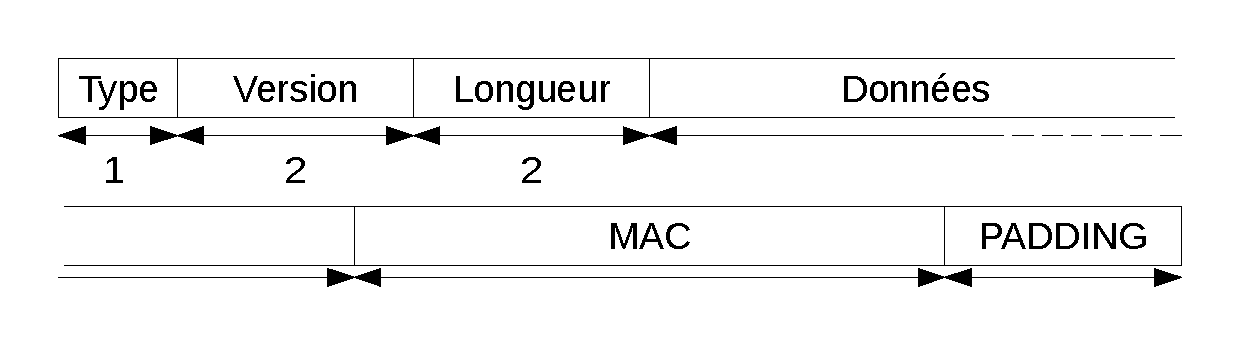
\includegraphics[scale=0.5]{schemaSSL2.pdf}
  \caption{Schéma d'un paquet SSL}
  \label{fig:ssl}
\end{figure}


Type :
\begin{itemize}
\item 0x16 : Handshake
\item 0x14 : Change Cypher Spec
\item 0x15 : Alert
\item 0x17 Application Data
\end{itemize}

Version :
\begin{itemize}
\item 0x3000 : SSLv3
\item 0x30xy : TLSvx.y
\end{itemize}

MAC :
\begin{itemize}
\item SHA1 : 20 octet de MAC
\item SHA256 : 32 octet de MAC
\item \dots
\end{itemize}
Les données sont chiffrées et leurs tailles est indiquées par
la longueur.

\section{Fonctionnement}
\label{sec:fct}

Le premier prés requis à satisfaire est de réussir à injecter du code sur le client. Ce code lui permet 
de forger les requêtes à envoyer au serveur. Le seul changement sur les requêtes sera l'ajout de caractère pour
aligner correctement l'entête afin que l'octet qu'il cherche soit en fin de bloc.

Pour rappel, un message chiffré par DES est découpé en bloc de 8 octets alors qu'avec AES, les blocs feront 16 octets. Dans la suite, nous considérerons l'utilisation d'un chiffrement DES.\\ 

L'attaquant cherchant à trouver le dernier octet du cookie de session va envoyer, via son script, la requête suivante :

\begin{figure}[h]
\label{fig:packet1}
\centering
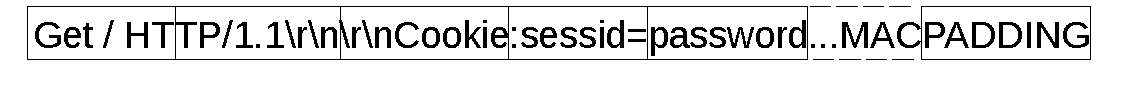
\includegraphics[scale=0.5]{Packet1}
\caption{Paquet envoyé}
\end{figure}

Il intercepte alors le paquet chiffré, prend le bloc contenant "password" puis le recopie à la
place du bloc de padding. Il envoie ce paquet modifié au serveur. 

 A la rececption du paquet, le serveur le déchiffre. Ensuite, il regarde le dernier octet du padding, qui corespond
à sa taille, et vérifie qu'il est inférieur à la taille d'un bloc. Il ne regarde pas le contenu du padding.
Dans notre cas, le padding occupant un bloc entier, son dernier octet sera $0x07$. A partir de cette longueur, 
il détermine la position des différentes parties du message. Il peut alors calculer le hashé des données et le comparer au MAC.

Pour que le paquet soit accepté il faut que le hashé des données corresponde au MAC et par extension, que la taille 
du padding soit correcte.

Notre requête modifiée ne sera acceptée que si le déchiffrement de l'octet recherché vaut $0x07$. Si ce n'est pas 
le cas, le serveur rejette le paquet et met fin à la connexion. Le script doit alors renégocier une clé avec le
serveur puis l'attaquant recommence avec le même clair.\\

 La requête a une chance sur 256 d'être acceptée, et cela indépendament des autres requêtes. Une fois qu'elle est
acceptée, il est possible de déterminer la valeur de l'octet recherché grâce au calcul suivant
\[ P_i[7] = 7 + C_{n-1}[7] + C_{i-1}[7] \]
avec i le numéro du bloc contenant "password" et n le nombre de bloc.

Pour s'attaquer à l'octet suivant, il faut simplement réaligner la requête comme ci-dessous :

\begin{figure}[h]
\label{fig:packet2}
\centering
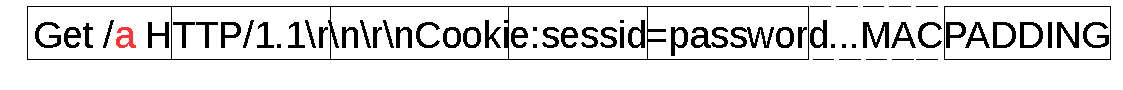
\includegraphics[scale=0.5]{Packet2}
\caption{Paquet envoyé}
\end{figure}

Il s'agit maintenant pour l'attaquant de réitérer l'oppération jusqu'à trouver l'ensemble du cookie.

\section{Implémentation}
\label{sec:imp}

Nous avons en premier lieu implémenté cette attaque dans un contexte TCP. A l'instar de \emph{SSL\_write()} qui gère le 
chiffrement et l'envoi d'un message, nous chiffrons ce dernier avant de l'envoyer via une connexion TCP.
Nous faisons donc le déchiffrement et les vérifications nous-mêmes et décidons des réponses envoyées au client.
C'est un modèle théorique qui nous a permis l'attaque d'un point de vue purement cryptographique. \\


Poodle étant basé sur POA, nous avons tout  d'abord implémenté ce dernier avec notre modèle.

 Le client chiffre son
message, remplace le dernier bloc par le bloc contenant l'octet recherché et modifie le dernier octet de l'avant-dernier bloc avant de l'envoyer au serveur. Celui-ci le déchiffre et vérifie si la taille du padding est correct. Si
tel est le cas, il envoie le message "VALIDE" au client, qui calcule alors l'octet recherché et passe au suivant.
Sinon, il répète l'opperation jusqu'à recevoir "VALIDE".\\

De cette première implémentation, nous avons enchainé sur celle de POODLE. Cette fois, nous avons trois acteurs,
Alice, Bob et Oscar. Alice chiffre son message et l'envoie à Oscar. Celui-ci le récupére, remplace le dernier bloc
comme pour POA et le retransmet imédiatement à Bob. Ce dernier procéde comme le serveur de POA. Si Alice reçoit
"INVALIDE", elle renégocie la clé et renvoie le même message. Sinon elle décale son message pour récupérer le 
prochain octet et procéde comme précédement.\\

Nous avons tenté d'implémenter cette attaque dans un vrai contexte SSL. L'idée est faire un programme qui permet à
Oscar de récupérer les messages transmis entre Alice et Bob et de le modifier si besoin. Il est capable de filtrer
les messages en fonctions de leurs types SSL (voir plus haut). Il va donc laisser passer le Handshake et ne s'intéressé qu'au type \emph{Application Data}. Il forge une requête avec le contenu du paquet qu'il reçoit et modifie le
bloc de padding comme d'habitude avant de l'envoyer. Pour éviter les problèmes de numéro de séquence, Oscar rejete 
au niveau du firewall, les paquets en provenance d'Alice et à destination de Bob.

Pour diverses raisons, ce modèle n'a pu être finalisé. En effet, lorsque Bob recevait un message erroné,
la renégociation de clé ne se faisait pas entre lui et Alice. Cela avait pour conséquence d'avorter l'attaque
dès le premier paquet modifié\\

Si besoin, notre code source est disponible sur GitHub : \url{https://github.com/StewieSuivant/Programmation-SSL}.
